%%%%%%%%%%%%%%%%%%%%%%%%%%%%%%%%%%%%%%%%%
% Beamer Presentation
% LaTeX Template
% Version 1.0 (10/11/12)
%
% This template has been downloaded from:
% http://www.LaTeXTemplates.com
%
% License:
% CC BY-NC-SA 3.0 (http://creativecommons.org/licenses/by-nc-sa/3.0/)
%
%%%%%%%%%%%%%%%%%%%%%%%%%%%%%%%%%%%%%%%%%

%----------------------------------------------------------------------------------------
%	PACKAGES AND THEMES
%----------------------------------------------------------------------------------------

\documentclass[UTF8,aspectratio=169,14pt]{ctexbeamer}

\usepackage{hyperref}
\hypersetup{
	colorlinks=true,
	linkcolor=red,
	anchorcolor=blue,
	citecolor=green
}

\mode<presentation> {
	
	% The Beamer class comes with a number of default slide themes
	% which change the colors and layouts of slides. Below this is a list
	% of all the themes, uncomment each in turn to see what they look like.
	
	%\usetheme{default}
	%\usetheme{AnnArbor}
	%\usetheme{Antibes}
	%\usetheme{Bergen}
	%\usetheme{Berkeley}
	%\usetheme{Berlin}
	%\usetheme{Boadilla}
	%\usetheme{CambridgeUS}
	%\usetheme{Copenhagen}
	%\usetheme{Darmstadt}
	%\usetheme{Dresden}
	%\usetheme{Frankfurt}
	%\usetheme{Goettingen}
	%\usetheme{Hannover}
	%\usetheme{Ilmenau}
	%\usetheme{JuanLesPins}
	%\usetheme{Luebeck}
	\usetheme{Madrid}
	%\usetheme{Malmoe}
	%\usetheme{Marburg}
	%\usetheme{Montpellier}
	%\usetheme{PaloAlto}
	%\usetheme{Pittsburgh}
	%\usetheme{Rochester}
	%\usetheme{Singapore}
	%\usetheme{Szeged}
	%\usetheme{Warsaw}
	
	% As well as themes, the Beamer class has a number of color themes
	% for any slide theme. Uncomment each of these in turn to see how it
	% changes the colors of your current slide theme.
	
	%\usecolortheme{albatross}
	%\usecolortheme{beaver}
	%\usecolortheme{beetle}
	%\usecolortheme{crane}
	%\usecolortheme{dolphin}
	%\usecolortheme{dove}
	%\usecolortheme{fly}
	%\usecolortheme{lily}
	%\usecolortheme{orchid}
	%\usecolortheme{rose}
	%\usecolortheme{seagull}
	%\usecolortheme{seahorse}
	%\usecolortheme{whale}
	%\usecolortheme{wolverine}
	
	%\setbeamertemplate{footline} % To remove the footer line in all slides uncomment this line
	%\setbeamertemplate{footline}[page number] % To replace the footer line in all slides with a simple slide count uncomment this line
	
	%\setbeamertemplate{navigation symbols}{} % To remove the navigation symbols from the bottom of all slides uncomment this line
}

\usepackage{graphicx} % Allows including images
\graphicspath{{./figs/}}
\usepackage{booktabs} % Allows the use of \toprule, \midrule and \bottomrule in tables
\usepackage{longtable}
\usepackage{listings}
\usepackage{xcolor}
\lstset{numbers=left, %设置行号位置
	numberstyle=\tiny, %设置行号大小
	keywordstyle=\color{blue}, %设置关键字颜色
	commentstyle=\color[cmyk]{1,0,1,0}, %设置注释颜色
	frame=single, %设置边框格式
	escapeinside=``, %逃逸字符(1左面的键),用于显示中文
	%breaklines, %自动折行
	extendedchars=false, %解决代码跨页时,章节标题,页眉等汉字不显示的问题
	xleftmargin=2em,xrightmargin=2em, aboveskip=1em, %设置边距
	tabsize=4, %设置tab空格数
	showspaces=false %不显示空格
}
% Fonts
% \usepackage{libertine}
% \setmonofont{Courier}
\setCJKsansfont[ItalicFont=Noto Serif CJK SC Black, BoldFont=Noto Sans CJK SC Black]{Noto Sans CJK SC}


%----------------------------------------------------------------------------------------
%	TITLE PAGE
%----------------------------------------------------------------------------------------

\title[第1讲]{第1讲 :操作系统概述} % The short title appears at the bottom of every slide, the full title is only on the title page
\subtitle{第一节:课程概述\&教学安排}
\author{向勇、陈渝、李国良} % Your name
\institute[清华大学] % Your institution as it will appear on the bottom of every slide, may be shorthand to save space
{
清华大学计算机系 \\ % Your institution for the title page
\medskip
\textit{xyong,yuchen@tsinghua.edu.cn} % Your email address
}
\date{\today} % Date, can be changed to a custom date

\begin{document}

\begin{frame}
\titlepage % Print the title page as the first slide
\end{frame}

%\begin{frame}
%\frametitle{提纲} % Table of contents slide, comment this block out to remove it
%\tableofcontents % Throughout your presentation, if you choose to use \section{} and \subsection{} commands, these will automatically be printed on this slide as an overview of your presentation
%\end{frame}
%
%%----------------------------------------------------------------------------------------
%%	PRESENTATION SLIDES
%%----------------------------------------------------------------------------------------
%
%%------------------------------------------------
%\section{第二节:教学安排} % Sections can be created in order to organize your presentation into discrete blocks, all sections and subsections are automatically printed in the table of contents as an overview of the talk
%%------------------------------------------------
\begin{frame}
    \frametitle{课程信息}
    \begin{itemize}
        \item 主讲教师:
        \begin{itemize}
            \item 陈渝
            \item 向勇、李国良
        \end{itemize}
        %\pause
        
        \item 助教: 
        \begin{itemize}
            \item 张译仁、钮泽平
        \end{itemize}
    \end{itemize}
\end{frame}

\begin{frame}
    
    \frametitle{预备知识}
    
    \begin{itemize}
        
        \item 程序设计语言(汇编、C和Rust)
        \begin{itemize}
            \item :( 不是开发应用程序
            \item :) 而是开发系统程序
            %\pause
        \end{itemize}
        \item 数据结构
        \begin{itemize}
            \item :) 理解基本数据结构即可 
        \end{itemize}
        %\pause
        \item 计算机组成原理
        \begin{itemize}
            \item :( 刘总/康总的RISC-V/x86/ARM/MIPS原理 
            \item  :)  \href{http://crva.ict.ac.cn/documents/RISC-V-Reader-Chinese-v2p1.pdf}{Patterson的RISC-V原理}
        \end{itemize}
        %\pause
        \item 编译原理
        \begin{itemize}
            \item :) 没学过影响不大  
            \item :( 但还是要了解高级语言<-->RISC-V汇编语言
            
        \end{itemize}
        
    \end{itemize}
    
\end{frame}

\begin{frame}
    \frametitle{课程信息}
    \begin{itemize}
        \item \href{http://os.cs.tsinghua.edu.cn/oscourse/OS2021spring}{课程\textbf{WIKI}}
        \begin{itemize}
            \item 所有课程信息的入口,也是最新课程信息的官方发布网站
        \end{itemize}
        %\pause
        \item 课程视频
        \begin{itemize}
            \item \href{https://next.xuetangx.com/}{学堂在线}:操作系统(RISC-V)
        \end{itemize}
        %\pause
        \item 作业
        \begin{itemize}
            \item \href{http://learn.tsinghua.edu.cn/f/wlxt/index/course/teacher/course?wlkcid=2019-2020-2140259621}{网络学堂 -- 向老师、李老师}		
            \item \href{http://learn.tsinghua.edu.cn/f/wlxt/index/course/teacher/course?wlkcid=2019-2020-2140259622}{网络学堂 -- 陈老师}
        \end{itemize}
        %\pause
        \item 云实验环境
        \begin{itemize}
            \item \href{https://www.shiyanlou.com/courses/1481}{rcore os在线实验环境}
            \item rcore tutorial云实验环境:ssh -l rcore 166.111.131.12
        \end{itemize}
        \item 讨论区
        \begin{itemize}
            \item \href{https://piazza.com/tsinghua.edu.cn/spring2015/30240243x/home}{Piazza交流论坛}
            \item 微信:OS2021
        \end{itemize}
    \end{itemize}
\end{frame}
%-------------------------------------------------
\begin{frame}
	\frametitle{参考教材}
	
%	\begin{columns}
%		
%		\begin{column}{0.5\textwidth}
			\textbf{参考教材}
			\begin{itemize}
				\item \href{http://www.ostep.org/}{Operating Systems: Three Easy Pieces \\ 操作系统:三大简易元素}
				\item \href{http://item.jd.com/10553956.html}{Operating System Concepts \\ 操作系统概念}
				\item \href{http://item.jd.com/10255221.html}{Operating Systems:Internals and Design Principles \\ 操作系统:精髓与设计原理}
			\end{itemize}
			\pause
		
			\textbf{上课时间地点}
			\begin{itemize}
				\item 星期一(1-13周) 上午 第2大节  09:50-11:25  五教5105、六教6A214
				\item 星期四(1-13周) 上午 第1大节  08:00-09:35  五教5105、六教6A214
		    \end{itemize}
%		\end{column}
%		
%		\begin{column}{0.5\textwidth}
%			
%			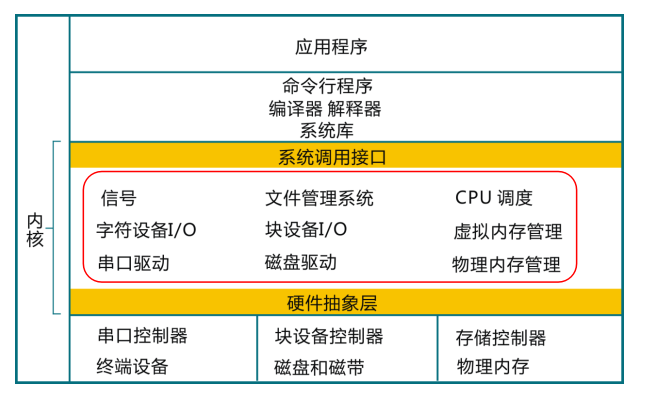
\includegraphics[width=1\linewidth]{ucore-arch}
%			
%		\end{column}
%		
%	\end{columns}
	
\end{frame}

%------------------------------------------------
\begin{frame}
	\frametitle{教学内容}

	\begin{columns}

	\begin{column}{0.5\textwidth}
	
    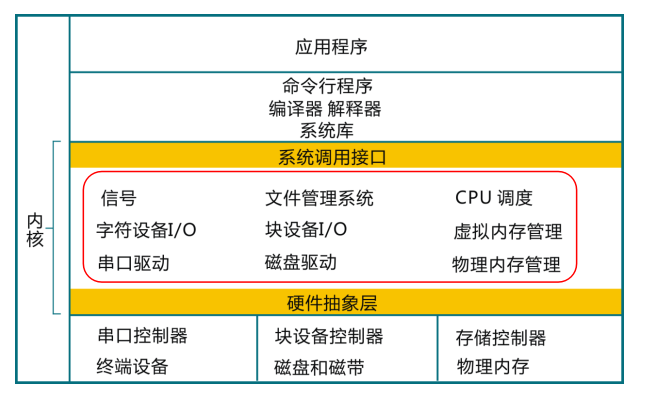
\includegraphics[width=1\linewidth]{ucore-arch}
    
    \end{column}
	
	\begin{column}{0.5\textwidth}
	\textbf{操作系统原理与实现}
    \begin{itemize}
		\item 操作系统结构
		\item 中断及系统调用 %\pause
		\item 内存管理
		\item 进程管理
		\item 处理机调度
		\item 同步互斥 %\pause
		\item 文件系统
		\item I/O子系统
    \end{itemize}
    
    \end{column}

\end{columns}

\end{frame}

%------------------------------------------------

    \begin{frame}
        \frametitle{作业与实验}
        \begin{itemize}
            \item 平时作业
        \begin{itemize}
    		\item 课上练习与交流
	    	\item 课后练习
        \end{itemize} %\pause

            \item 基础实验
    \begin{itemize}
		\item r/u Core实验:面向RISC-V CPU用Rust/C写操作系统
    \end{itemize}
            \item 课程设计(大实验)
        \end{itemize}
\end{frame}

%------------------------------------------------
\begin{frame}
\frametitle{基础实验}
\framesubtitle{Core实验:面向RISC-V CPU用Rust/C写操作系统} %\pause
\begin{columns}
	
\begin{column}{0.5\textwidth}
\begin{itemize}
		\item 实验零:操作系统实验准备
		\item 实验一:hello-world OS
		\item 实验二:kernel-mode OS
		\item 实验三:multi-programming OS
		\item 实验四:mem-isolation OS
\end{itemize}
\end{column}
 
\begin{column}{0.5\textwidth}
    \begin{itemize}
		\item 实验五:multi-process OS
		\item 实验六: Inter-Process-Comm OS
		\item 实验七:File-System OS
		\item 实验八:r/u Core OS
	\end{itemize}
\end{column}

\end{columns}

\end{frame}



%------------------------------------------------
\begin{frame}
\frametitle{课程设计}
	\begin{itemize}
	\item 各种CPU平台上的操作系统移植
		\begin{itemize}	
		\item RISC-V、x86-64、x86-32、MIPS、ARM
		\end{itemize}
	\item 操作系统内核功能实现和扩展
		\begin{itemize}	
		\item GUI、驱动、内核可加载模块、微内核
		\end{itemize} \pause
	\item 操作系统分析工具	
		\begin{itemize}	
		\item 错误分析、行为分析、模拟器
		\end{itemize}
	\item 操作系统新方向探索
		\begin{itemize}	
		\item Rust、内核语言
		\end{itemize} \pause
	\item \href{https://github.com/oscomp/os-competition-info}{第一届全国全国大学生操作系统设计比赛}
		\begin{itemize}	
		\item \href{https://github.com/oscomp/proj2-os-kernels-by-history}{挖掘历史的OS kernel生物群}
        \item \href{https://github.com/oscomp/proj9-zcore}{探索未来的OS Kernel -- zCore}
		\end{itemize}
	\end{itemize}
\end{frame}
%------------------------------------------------
    
\begin{frame}[fragile]
    \frametitle{成绩评定}
    \begin{itemize}
        %\item 作业:5分
        \item 实验:30分
        \begin{itemize}
            \item 独立完成操作系统实验,并提交实验报告
        \end{itemize} %\pause
        \item 考试或课程设计:70分
        \begin{itemize}
            \item 期中考试:30分
            \item 期末考试:40分
            \item 有余力和兴趣的同学,可用课程设计替代考试
        \end{itemize}

    \end{itemize} %\pause

    总成绩加权方法:上述各项成绩的总和会做一次调整,基本原则是,各分数段保持一定的比例,可能的参考比例为A+/A/A-占25\%、B+/B/B-占45\%、C+/C/C-占20\%和D+/D/F占10\%。 
    \newline \newline
    
    详见:\href{http://os.cs.tsinghua.edu.cn/oscourse/OS2020spring/log#A20200210-.2BZM1PXHz7ft.2BL.2FnoLdoRiEH7pi8RbmmgHUcaL9GYO-}{去年的操作系统课程的成绩评定标准说明:会调整!!!}
    
\end{frame}

%------------------------------------------------
    
    \begin{frame}
        \frametitle{调查问卷}
        \begin{itemize}
            \item 为什么要学这门课? %\pause
            \item 你打算如何来学这门课?
            \item 对自己的课程学习要求是什么?
            \item 你愿意如实报告是否独立完成实验任务?
            \item 你希望在操作系统课上学到什么知识和什么能力? %\pause
            \item 以前的学习情况?
            \item 对计算机专业的看法是什么? %\pause
            \item 采集仅限于操作系统课内注册的同学信息
        \end{itemize}
    \end{frame}
%----------------------------------------------------------------------------------------

\end{document}
